\documentclass[12pt]{article}

\usepackage[margin=1in]{geometry}
\usepackage{amsmath}
\usepackage{amsthm}
\usepackage{graphicx}
\usepackage[utf8]{inputenc}
\usepackage{hyperref}
\hypersetup{colorlinks = true, linkcolor = blue, citecolor=blue, urlcolor = blue}
\usepackage{natbib}
\usepackage{enumitem}
\usepackage{setspace}
\usepackage{lipsum}
\usepackage{wrapfig}
\usepackage{algorithm}
\usepackage{algpseudocode}
\usepackage{tikz}

\title{Fake Amazon reviews detection using natural language processing and supervised learning}

\author{Michael Zheng\\
  Jun Yan\\[1ex]
  Department of Statistics, University of Connecticut\\
}
\date{}

\begin{document}
\maketitle
\doublespace

\begin{abstract}
    Customer reviews play an important role of influencing one's purchase decision. Consumers trust the reputation of the brand or product based on reviews, while sellers are interested in making sales. Positive reviews can increase sales, and negative reviews can hamper sales. Thus, sellers can, and often do, abuse the review system for their own gain. They can do this by generating artificial positive reviews for themselves to bolster their brand's reputation or negative reviews for their competitors to reduce their competitor's sales. This paper seeks to develop a support vector machine model to accurately detect these artificially created Amazon reviews using natural language processing techniques. The paper also investigates other ways in which malicious reviews can exist, such as vendors encouraging their customers to write positive reviews for them in exchange for money or goods. Finally, the approach taken in this paper is very simple and more complex methods that yield higher detection accuracy already exist in the literature. This paper only seeks to corroborate the idea that supervised learning is an effective technique to classify fake reviews. The paper ends with an explanation of the limitations of the study and potential future works.
    
\bigskip
\noindent{\sc Keywords}:
natural language processing;
sentiment analysis;
supervised learning;
support vector machine.

\end{abstract}

\section{Introduction}
\label{sec:intro}

Reviews are an integral part of an Amazon customer's shopping experience. They can, and often are, abused by sellers to promote their own products or stifle competition. Products with good ratings and feedback are deemed to be more trustworthy and help increase sales, while negative reviews discredit the product and hurt sales. The sheer volume of reviews that are published daily make them difficult to moderate manually. Furthermore, there has been more awareness about fake reviews in the last few years and those behind them have an incentive to write increasingly realistic ones. However, fake reviews are ultimately generated using a systematic approach and thus contain elements that differentiate them from genuine reviews \citep{Salminen2022}. A machine learning model, unlike a human, can learn in real-time and adapt to new techniques used to generate fake review in order to accurately classify them. With so much to gain and little to lose for vendors, it's important to detect fake reviews from genuine ones in order to make the Amazon marketplace fair \citep{Salminen2022}.

Sentiment analysis is a method of quantifying positive, neutral, or negative opinions to a piece of text. Reviews can be assigned an opinion type based on the presence of certain words. For instance, the words "fantastic" and "useless" are associated with a positive and negative experience with a product, respectively. Thus, reviews that are written to promote a product are positive in nature, while those written to demote a product, usually by a competitor, are negative \citep{pendyala_2019}.

Previous studies, such as this one carried out by \citep{article}, demonstrated success in detecting fake reviews using sentiment analysis and supervised learning to classify reviews. However, reviews in their raw form cannot be interpreted by classification models. They must be processed by removing stopwords, commonly used English words such as "a" and "the", and then tokenized by splitting sentences into smaller fragments that can be more easily assigned meaning by machine learning models. 

There are several challenges about using sentiment analysis to detect fake reviews. Firstly, words can have a different connotation in a review depending on the type of product. The word "long", for example, would be a positive sentiment regarding a light bulb's life span. But if it was used to describe a hard drive's write speed, then it would be a negative sentiment. Secondly, fake reviews refer to reviews that are created by a non-human entity, such as text generators, to maliciously promote one's own product or demote a competitors. Vendors can also incentivize buyers to leave positive reviews about their products by offering the buyers endorsements or other perks. Even though these reviews were generated by a human entity, they should still be considered fake reviews because they are positive in light and used to promote more sales of the product and ultimately don't reflect the honest opinions of the buyer \citep{Salminen2022}.

The main contribution of this paper is to corroborate the findings of prior research papers on this topic. That is, NLTK, an open source natural language processing framework, will be used to process Amazon reviews by removing stopwords and tokenizing sentences because prior studies have shown this is an effective way to detect fake reviews. Then, a support vector machine (SVM), a popular supervised learning technique for classification problems, will be trained using a Amazon reviews dataset from Kaggle to detect fake reviews in a test set \citep{kr.goyal_keswani_goyal}.

\begin{wrapfigure}{l}{0.25\textwidth}
    \centering
    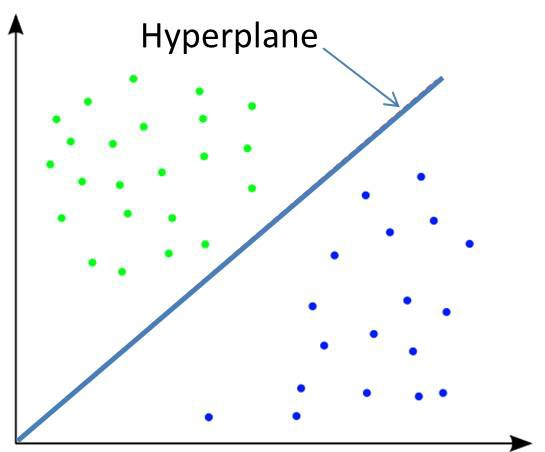
\includegraphics[width=0.25\textwidth]{manuscript/svm.jpg}
\end{wrapfigure}
A support vector machine or SVM is a machine learning algorithm that finds a
hyperplane that lies in the space of the input data and optimally divides the data points into 2 classes depending on which side of the hyperplane the points lie. For the purposes of this paper, an SVM will be used to classify Amazon reviews data as "fake" (ex. blue points) or "real" (ex. green points) \citep{Evgeniou2001}.

The paper will be organized as followed: Section 2 provides a description of the dataset used. Section 3 presents the methodology. Section 4 discusses the results of the study. Section 5 presents the conclusion, limitations, and future works.

\section{Data Collection}
\label{sec:data}

The data that will be used for this paper contains 21,000 Amazon reviews from 2018 across a number of product categories. The reviews are labelled as either a fake or real review. Each review has a corresponding rating and review title as well. There is also product metadata consisting of the product category and product title. This dataset was sourced from \href{https://www.kaggle.com/datasets/lievgarcia/amazon-reviews}{Kaggle}. 

The dataset contains features and corresponding labels for training and testing a support vector machine (SVM) to detect fake Amazon reviews. In total, there are 9 columns, 7 are categorical and 2 are numerical. 

\bigskip
\bigskip

\begin{tabular}{ |p{3cm}||p{3cm}|p{3cm}|p{3cm}|  }
 \hline
 \multicolumn{4}{|c|}{Dataset} \\
 \hline
 Variable& Data Type &Instance &Purpose\\
 \hline
 Doc-ID&Int&1, 2, 3, 4, 5, ...&Index\\
 Label&Str&label1, label2&Data Labels (y)\\
 Rating&Int&1, 2, 3, 4, 5&Feature (x)\\
 Verified-purchase&Str&N, Y&Feature (x)\\
 Product-category&Str&PC, Wireless, ...&Feature (x)\\
 Product-ID&Str&B00008N...&Feature (x)\\
 Product-title&Str&Targus...&Feature (x)\\
 Review-title&Str&Great com...&Feature (x)\\
 Review-text&Str&I was lookin...&Feature (x)\\
 \hline
\end{tabular}

\bigskip
\bigskip

\caption{Figure: The 'variable' column shows the names of all the variables that are in the dataset. The 'Data Type' column shows the data type of each variable in the dataset. Note that 'Int' means integer and 'Str' means string. The 'Instance' column shows an example of what a data point for that column would look like. The 'Purpose' column shows the importance of each variable to the machine learning step.}

The data was explored and visualized using the pandas library in Python. Specifically, each variable was grouped by the label, which is a 0 if the review is real and a 1 if the review is fake, to assess the frequency of the values of each variable in the fake and real reviews. This provided information about which products were over or under-represented so that the dataset could be balanced to avoid bias to the majority classes.

\section{Methods}
\label{sec:methods}
The data was processed to remove irrelevant or redundant information. A simple approach to sentiment classification was attempted. Any rating that is greater than 3 stars was assigned a value of 1 and was attributed to a positive opinion. Concurrently, ratings that are exactly 3 stars were negated as they were neutral opinions and the remaining ratings are assigned a 0 and considered a negative opinion. The number of usable data points was reduced from 21,000 to 19,132.

An imbalance between positively and negatively opinionated ratings was present. There were 16,183 positive ratings compared to just 2,949 negative ratings. 20\% of the ratings with a newly assigned value of 1 were randomly selected, which was approximately 3237 data points, to better balance them with the number of 0 ratings, 2949. The imbalance was addressed to ensure that the SVM model does not ignore the minority class and overfit to the majority class, resulting in a model that is better able to generalize to new instances. This resulting subset of the dataset contains 6,186 data points and was used for further processing.

The review text was processed by removing stop words, which are commonly used English words. For instance, the root word of "running" is "run", which the NLTK framework can recognize and remove the "ing". This is done to ensure that the SVM model only focuses on the important information of a word. This is done for each word in a review for every review in the dataset in a process called lemmatization. With each review converted to a list of words in its base form, bigrams, or pairs of English words that commonly go together, were generated for each possible pair of words in the list. These bigrams convey more information about the general sentiment of the reviews through the frequency of such pairs occurring in a body of text.

\bigskip
\bigskip

\begin{center}
\begin{tabular}{ |c|c|c|c| } 
\hline
Original Sentence & Stop Words & Lemmatization & Bigrams \\
\hline
\multirow I like playing with cats & I, like, with & play, cat & (play, game), (cute, cat) \\
\hline
\end{tabular}
\end{center}

\bigskip

\caption{Figure: This figure showcases an example of how the natural language processing techniques used in this study works. Suppose an Amazon review reads as follows: I like playing with cats. The words I, like, and with are commonly used in English sentences. They are called stop words and contain no important information about the sentiment of the review. The algorithm will remove these words. The most meaningful words playing and cat remain. But we want to ensure that these words are in their base form so that they can convey the most information to the machine learning algorithms that we feed them into. Thus, playing becomes play and cat stays as cat, since its already in its base form. Finally, we find words that commonly go together with play and cat and generate what we call, bigrams. The word game is commonly used with play and the word cute is commonly used with cat.}

\bigskip

Several models were attempted using different feature vectorization approaches and natural language processing techniques in an attempt to find the best performing model. For instance, in one approach, all the features were included and a SVM model was trained. But the performance was poor at approximately 47$\%$ accuracy, which is worse than randomly guessing. This was most likely due to extra noise being generated from the Product-ID feature, which conveys no information about fake reviews. Since it is simply an ID used to uniquely identify each product, the feature distracted the SVM model from properly defining the classification boundary.

Features that were deemed to irrelevant to detecting fake reviews were removed, such as Doc-ID, Label, Product-ID, Product-title, and Review-title. The features that were kept included the rating, verified purchase status, product category, and review. These features were stored in a feature vector for each observation alongside its corresponding label. This was done to numerically quantify the contents of the categorical variables so that the SVM model, which requires numerical input features, can use them to make predictions. A simple feature vectorization approach was utilized for the purposes of this paper. 

\bigskip

\begin{algorithm}
\caption{Feature Vectorization}\label{alg:feature-vector}
\begin{algorithmic}
\State $X$: a set of feature information

    \Procedure{Feature Vector}{Rating, Verified-Purchase, Product-Category, Review}
    \State $X_{1} = Rating$
    \bigskip
    
    \If {\textit{Verified-Purchase} = "Y"}
        \State $X_{2} = 1$
    \Else
        \State $X_{2} = 0$
    \EndIf
    \bigskip
    
    \If {\textit{Product-Category} \textbf{not in} X}
        \State $X_{3} = 1$
    \Else
        \State $X_{3} \mathrel{{+}{=}} 1$
    \EndIf
    \bigskip

    \For{each word $w$ in $Review$}
        \If {\textit{w} \textbf{not in} X}
            \State $X_{4} = 1$
        \Else
            \State $X_{4} \mathrel{{+}{=}} 1$
        \EndIf
    \EndFor
    \bigskip
    
    \State \textbf{return} $X$
    
    \EndProcedure

\end{algorithmic}
\end{algorithm}

\caption{Figure: The feature vectorization algorithm takes an input vector X that contains 4 features: rating, verified-purchase, product-category, and review. The idea is to convert any non-integer type variable into a numerical value so that the machine learning algorithm can make sense of it. The rating ranges from 1 to 5 and contains good information by itself. If the rating is 1, we know the customer had a bad experience. Otherwise, the experience becomes increasingly better as it approaches 5, with 5 being the best. The verified-purchase variable is a binary variable with the values "Yes" and "No". Thus, we can represent "Yes" with a value of 1 and "No" with a value of 0. The product-category, on the other hand, is slightly different. If the product category has not been seen before by the algorithm, then a value of 1 is assigned to it. Otherwise, for each occurrence of this product-category, we add 1 to the current value and assign that new value to product category. (For example, if a product category currently has a value of 5 and in the given feature vector it occurs again, then the value of the product category will be 6). This ensures that their is an understandable importance of product categories by the SVM model. That is, a product category with a higher value is emphasized since it occurs more frequently. We approach the review text in a similar fashion. The value assigned to each word is initially 0 and incremented by 1 every time it occurs again. This is to, once again, emphasize the importance of frequency.}

The data was then split into a test and training set based on a proportion $p$, which is the proportion of data from the 6,186 data points to devote to the training set. For the results generated in this paper, 80\% of the data was randomly assigned to the training set and the rest were used as a test set \citep{bell_2020}. The proportion $p$, which is the size of the training set, was arbitrarily chosen to be greater than the size of the testing set $(1-p)$ to ensure that the SVM model is trained on as much data as possible to find and learn meaningful patterns. It is widely accepted for training data to be larger than testing data. An inadequate amount of training data can result in a poor performing model that underfits and does not generalize to new instances well.

A SVM model was fitted to the training data and then validated on the test set using the scikit-learn library in Python. Several performance metrics about the predictions were then assessed.

\bigskip
\bigskip
\bigskip

\usetikzlibrary{positioning,fit}
\makeatletter
\pgfkeys{/pgf/.cd, % from https://tex.stackexchange.com/a/12039/121799
  parallelepiped offset x/.initial=2mm,
  parallelepiped offset y/.initial=2mm
}
\pgfdeclareshape{parallelepiped}
{
  \inheritsavedanchors[from=rectangle] % this is nearly a rectangle
  \inheritanchorborder[from=rectangle]
  \inheritanchor[from=rectangle]{north}
  \inheritanchor[from=rectangle]{north west}
  \inheritanchor[from=rectangle]{north east}
  \inheritanchor[from=rectangle]{center}
  \inheritanchor[from=rectangle]{west}
  \inheritanchor[from=rectangle]{east}
  \inheritanchor[from=rectangle]{mid}
  \inheritanchor[from=rectangle]{mid west}
  \inheritanchor[from=rectangle]{mid east}
  \inheritanchor[from=rectangle]{base}
  \inheritanchor[from=rectangle]{base west}
  \inheritanchor[from=rectangle]{base east}
  \inheritanchor[from=rectangle]{south}
  \inheritanchor[from=rectangle]{south west}
  \inheritanchor[from=rectangle]{south east}
  \backgroundpath{
    % store lower right in xa/ya and upper right in xb/yb
    \southwest \pgf@xa=\pgf@x \pgf@ya=\pgf@y
    \northeast \pgf@xb=\pgf@x \pgf@yb=\pgf@y
    \pgfmathsetlength\pgfutil@tempdima{\pgfkeysvalueof{/pgf/parallelepiped offset x}}
    \pgfmathsetlength\pgfutil@tempdimb{\pgfkeysvalueof{/pgf/parallelepiped offset y}}
    \def\ppd@offset{\pgfpoint{\pgfutil@tempdima}{\pgfutil@tempdimb}}
    \pgfpathmoveto{\pgfqpoint{\pgf@xa}{\pgf@ya}}
    \pgfpathlineto{\pgfqpoint{\pgf@xb}{\pgf@ya}}
    \pgfpathlineto{\pgfqpoint{\pgf@xb}{\pgf@yb}}
    \pgfpathlineto{\pgfqpoint{\pgf@xa}{\pgf@yb}}
    \pgfpathclose
    \pgfpathmoveto{\pgfqpoint{\pgf@xb}{\pgf@ya}}
    \pgfpathlineto{\pgfpointadd{\pgfpoint{\pgf@xb}{\pgf@ya}}{\ppd@offset}}
    \pgfpathlineto{\pgfpointadd{\pgfpoint{\pgf@xb}{\pgf@yb}}{\ppd@offset}}
    \pgfpathlineto{\pgfpointadd{\pgfpoint{\pgf@xa}{\pgf@yb}}{\ppd@offset}}
    \pgfpathlineto{\pgfqpoint{\pgf@xa}{\pgf@yb}}
    \pgfpathmoveto{\pgfqpoint{\pgf@xb}{\pgf@yb}}
    \pgfpathlineto{\pgfpointadd{\pgfpoint{\pgf@xb}{\pgf@yb}}{\ppd@offset}}
  }
}
\makeatother
\begin{tikzpicture}[standard/.style={minimum width=3cm,draw,align=center},
font=\sffamily]
 \begin{scope}[local bounding box=boxes]
  \node[standard,minimum height=4cm] (TS) {Training Set};
  \node[standard,below=-\pgflinewidth\space of TS] (TeS) {Test Set};
  \path (TS.north west) -- (TS.north east) node[midway,above]{Dataset};
  \node[right=1.5cm of TeS.north east,standard] (T1) {Train};
  \node[right=-\pgflinewidth\space of T1,standard,minimum width=1cm] (TT1) {Test};
  \node[above=1.5cm of T1,standard] (T2) {SVM};
  \node[above=1.5cm of T2,align=center,inner xsep=1.5em] (PE) {Trained\\ model};
  \node[yscale=-1,parallelepiped,draw,fit=(PE),inner sep=0pt]{};
  \node[right=3cm of PE,standard] (PR) {Predictions};
  \node[below=1cm of PR,standard,rounded corners=1em] (CEM) {Calculate\\ evaluation\\ metrics};
 \end{scope}
 \begin{scope}[-latex,thick]
  \draw (TeS.east) -- (T1.west);
  \draw (T1) -- (T2) node[midway,right]{Feed the model};
  \draw[shorten >=1mm] (T2) -- (PE) node[midway,right]{Learning};
  \draw[shorten <=1mm] (PE) -- (PR);
  \draw (PR) -- (CEM);
  \draw[rounded corners] (TT1.east) -- ++ (2em,0) |- (CEM);
 \end{scope}
 \begin{scope}[nodes={text width=3.5cm,align=center}]
  \node[below] at (boxes.south-|TS) {Data pre-processed using feature vectorization.};
  \node[below] at ([xshift=5mm]T1|-boxes.south) {Train part fed to model. Test used for model validation};
  \node[below] at (CEM|-boxes.south) {Metrics using predictions and test labels.};
 \end{scope}
\end{tikzpicture}

\bigskip

\caption{Figure: We begin with a dataset that we devote 80$\%$ to a training set and 20$\%$ to a test set. The data are pre-processed by removing irrelevant features, applying natural language processing techniques, and utilizing feature vectorization. The training set is then fed into an SVM model through the scikit-learn, Python library. The model is trained on that data and is used to make predictions about the test set. We then compare the predictions to the true labels and calculate several evaluation metrics to assess the performance of the model.}

\bigskip

It is common practice to devote a chunk of the dataset to a validation set for a total of 3 sets: training set, validation set, and test set. This is useful for hyper-parameter optimization because when you fine-tune the hyper-parameters to get better model performance you don't want to overfit it to the test set. Otherwise, the evaluation metrics calculated will not accurately assess the generalizability of the model. Instead, we want to fine-tune the hyper-parameters of the model to perform well on the validation set. Then, if we are happy with the validation performance, we can evaluate the model's performance on the test set to gain insights about the generalization performance of the model. A validation set was not utilized in this study, but it is certainly something to look into in the future.

\section{Results}
\label{sec:results}

In this section, the results from the SVM model to classify fake and real Amazon reviews from the Kaggle dataset are presented. Accuracy, recall, and precision are common metrics to evaluate the performance of a classification model. Accuracy is "the degree of closeness between a measurement and its true value" \citep{admin_2022}. Precision is the "fraction of relevant instances among the retrieved instances" \citep{wikipedia_2022}. Recall is the "fraction of relevant instances that were retrieved" \citep{wikipedia_2022}. They can be calculated using the information in a confusion matrix, which is a 2x2 matrix where each row represents a review that is actually fake or real and each column represents a review that is predicted to be fake or real.

\bigskip
\bigskip

\scalebox{1.1}{%
\begin{tabular}{l|l|c|c|c}
\multicolumn{2}{c}{}&\multicolumn{2}{c}{Predicted Reviews}&\\
\cline{3-4}
\multicolumn{2}{c|}{}&Fake&Real&\multicolumn{1}{c}{Total}\\
\cline{2-4}
\multirow{Actual Reviews}& Fake & $717$ & $211$ & $928$\\
\cline{2-4}
& Real & $56$ & $254$ & $310$\\
\cline{2-4}
\multicolumn{1}{c}{} & \multicolumn{1}{c}{Total} & \multicolumn{1}{c}{$773$} & \multicolumn{    1}{c}{$465$} & \multicolumn{1}{c}{$1238$}\\
\end{tabular}}

\bigskip

\caption{Figure: This is a 2 dimensional confusion matrix visualizing the performance of the supervised SVM model's classification of fake Amazon reviews. The first row represents reviews that are actually fake reviews. The second row represents reviews that are actually real reviews. The first column represents reviews that are predicted to be fake. The second column represents reviews that are predicted to be real.}

\bigskip

\begin{itemize}
  \item True positives (TP) = predicted fake reviews $\cap$ actual fake reviews
  \begin{itemize}
    \item{The true positive value tells us the number of instances where the model properly predicts a review to be fake.}
  \end{itemize}
  \item True negatives (TN) = predicted real reviews $\cap$ actual real reviews
  \begin{itemize}
    \item{The true negative value tells us the number of instances where the model properly predicts a review to be real.}
  \end{itemize}
  \item False positives (FP) = predicted fake reviews $\cap$ actual real reviews
  \begin{itemize}
    \item{The false positive value tells us the number of instances where the model incorrectly predicts a review to be fake when it is actually real.}
  \end{itemize}
  \item False negatives (FN) = predicted real reviews $\cap$ actual fake reviews
    \begin{itemize}
    \item{The false negative value tells us the number of instances where the model incorrectly predicts a review to be real when it is actually fake.}
  \end{itemize}
  \item Positives (P) = total amount of actual fake reviews
    \begin{itemize}
    \item{The positive value tells us the number of actual fake reviews.}
  \end{itemize}
  \item Negatives (N) = total amount of actual real reviews
  \begin{itemize}
    \item{The negative value tells us the number of actual real reviews.}
  \end{itemize}
  \item Accuracy = (TP + TN) / (P + N)
    \begin{itemize}
    \item{Accuracy, as defined earlier, can be obtained by dividing the sum of true positives and true negatives by the sum of positives and negatives}
  \end{itemize}
  \item Precision = (TP) / (TP + FP)
  \begin{itemize}
    \item{Precision, as defined earlier, can be obtained by dividing the number of true positives by the sum of true positives and false positives}
  \end{itemize}
  \item Recall = (TP) / (TP + FN)
  \begin{itemize}
    \item{Recall, as defined earlier, can be obtained by dividing the number of true positives by the sum of true positives and false negatives}
  \end{itemize}
\end{itemize}

Accuracy is defined as the degree to which the model classifies all the reviews properly. In this case, the model classified 78.4$\%$ of the reviews in the test set properly. 

\[Accuracy = \dfrac{TP + TN}{P + N} = \dfrac{717 + 254}{928 + 310} = 0.784\]

Precision is a measurement of the exactness of the model's classifications. Here, the model predicted 773 reviews as being fake and of those, 92.7$\%$ of them were correct.

\[Precision = \dfrac{TP}{TP + FP} = \dfrac{717}{717 + 56} = 0.927\]

Recall, simply put, is the proportion of relevant instances that were correctly classified, which in this case would be fake reviews. This model classified 77.3$\%$ of the actual fake reviews as fake.

\[Recall = \dfrac{TP}{TP + FN} = \dfrac{717}{717 + 211} = 0.773\]

The SVM model performs better than a random guess with an accuracy of 78.4$\%$. The misclassification of fake reviews as real is more detrimental than the other way around because in the former scenario, potential customers will base their purchasing decisions on wrong information. Thus, the recall, or the ability of the model to identify fake reviews from the ones that are actually fake, should be maximized. For this model, the recall is at a reasonably high value of 77.3$\%$. Another thing that should be mentioned is the high precision. Specifically, when the model predicts that a review is fake, it is correct 92.7$\%$ of the time using this dataset.

Previous attempts at detecting fake Amazon reviews yielded a precision and recall as high as 0.97, respectively \citep{Salminen2022}. That represents a significant improvement over the model developed in this paper. Specifically, the model in that paper can detect actual fake reviews as fake 97$\%$ of the time with 97$\%$ certainty. The paper utilized the RoBERTa (Robustly Optimized BERT Pretraining Approach) model, which tends to outperform other classifiers in natural language processing tasks by training with larger mini-batches and learning rates \citep{https://doi.org/10.48550/arxiv.1907.11692}.

The results indicate that machines are effective at detecting fake reviews, especially when the data is properly pre-processed, desirable features are selected, and the most optimal model is used. The model developed for this paper has an accuracy of 78.4$\%$, which is (78.4 – 50)/50 = 56.8$\%$ better than a random guess. Therefore, this paper supports the results and ideas put forward by previous studies that machines are effective tools to detect fake Amazon reviews.

\section{Conclusion}
\label{sec:conclusion}
Detecting fake reviews is an ever-changing challenge because perpetrators are constantly seeking better methods of generating realistic, fraudulent reviews. It is impossible to efficiently filter the thousands of reviews being submitted every second on Amazon, manually. Machines are the next logical step for this process. This paper corroborates the methodologies and findings of prior research papers on this topic. Natural language processing and supervised learning techniques are effective methods of detecting genuine reviews from non-genuine ones. This is important because vendors acting in bad faith may create fake positive reviews to promote their products or generate fake negative reviews to stifle their competition. In theory, this model, like many similar models, may automate fake review detection and make the Amazon marketplace fair.

This study did not create any new features from the existing features, which may be beneficial to improving model performance. Feature engineering is the process of using domain knowledge to create new features that better explain the response variable so that, hopefully, the model performance can be improved. Specifically, a number of potentially useful features could be created from the review texts. For instance the number of emojis, capital letters, and punctuation marks used may convey more information about the sentiment of the customer. Furthermore, those same features can occur more or less frequently in fraudulent reviews and provide stronger classification separation in the SVM. 

Hyper-parameter tuning was also not utilized in this study, which may benefit generalization performance. Hyper-parameters are parameters that control the learning process of a machine learning model. For instance, defining the proper loss function ensures that we are measuring the correct metric in order to assess performance. It is imperative to find the optimal set of hyper-parameters in order to maximize model performance

Furthermore, the dataset used to train the SVM model in this paper is small (n = 6,186). The key to getting better, more robust performance is using a dataset that is balanced and sufficiently large (n = 40,000) \citep{Salminen2022}. This ensures that the model can discover the underlying trends and patterns of the data and make better class separation. Additionally, the techniques used to generate fake reviews vary over time as perpetrators and moderators engage in a game of cat and mouse. Thus, testing on a data that spans a longer time frame is crucial to not over-fitting the model to a specific interval of time. That is, by exposing the model to numerous fake review generation types, the model could learn trends, blind to the human eye, that are vital to detecting fake reviews, irrespective of time. A high performing, robust model for detecting fake reviews is important to ensuring an honest and trustworthy Amazon marketplace.

Ultimately, with the continued advancements in supervised learning techniques, there will be a future where reviews will no longer need to be manually vetted. Every review will be automatically processed by these models upon submission and only the genuine ones will be published, to a high degree of accuracy. Furthermore, with the growth of e-commerce, or online retail, the applications of these models should be extended beyond Amazon to other online shopping outlets, like eBay. Going forward, the largest hurdle to detecting fake reviews will not be in the realm of machine learning. It will be obtaining high-quality, labeled data sets to train models with. As it currently stands, obtaining these data sets is manual in nature and costly in terms of time and money. However, its important to put this into context. Researchers looking to study this topic may find it difficult to access good datasets. But the companies behind these online retail sites have troves of data that can be used for this purpose. It's also in their interest to keep their marketplace fair and clean of bad actors to maintain their reputation as a legitimate site to conduct business. Despite these difficulties, this study is a step forward into this future.

\bibliographystyle{chicago}
\bibliography{references.bib}

\end{document}
